\section{Infanterietrupp / Fireteam (FT)}
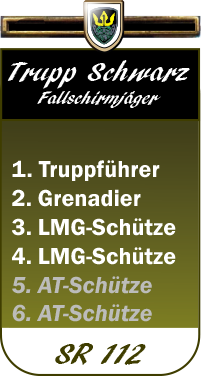
\includegraphics[width=20mm]{./img/truppenordnung/infanterie/infanterie.png}\\
Die Infanterie bildet den Kernbestandteil vieler Missionen. Ein Infanterietrupp ist immer Teil eines Zuges und besteht aus 4 oder 6 Mann. Mögliche Positionen innerhalb eines Infanterietrupps sind:
\begin{itemize}
	\item Truppführer (TF) / Fireteam Leader (FTL)
	\item Grenadier (GRE)
	\item Leichter MG-Schütze (LMG) / Automatic Rifleman (AR)
	\item Mittlerer MG-Schütze / Medium Machine Gunner (MMG)
	\item MG-Assistent / Assistant Machine Gunner (AMG) - notwendig für MMG
	\item Leichter Panzerabwehrschütze / Light Anti Tank (LAT)
	\item Schwerer Panzerabwehrschütze / Heavy Anti Tank (HAT)
	\item Panzerabwehr-Assistent / Assistant Anti Tank (AAT), notwendig für HAT
	\item Luftabwehrschütze / Anti-Air (AA)
	\item Pionier / Pioneer (PIO)
	\item Gefechtssanitäter / Combat Medic (CM)
\end{itemize}
Auf eine sinnvolle Einteilung in Buddy-Teams (z.B. bei Positionen, die einen Assistenten erfordern), ist hierbei zu achten.\\
Die Kommunikation erfolgt ausschließlich über Short-Range, der Truppführer schaltet sich über seine Additional-Short-Range auf den Zugkanal auf, um sich mit der Zugführung und den anderen Truppführern im Zug abzusprechen. Die Nummer 2 im Trupp kann sich ebenfalls auf den Zugfunk aufschalten, jedoch nur mithören und nicht funken - es sei denn, der Truppführer fällt aus und die Nummer 2 übernimmt.